% +--------------------------------------------------------------------+
% | Sample Chapter 3
% +--------------------------------------------------------------------+

\cleardoublepage

% +--------------------------------------------------------------------+
% | Replace "This is Chapter 3" below with the title of your chapter.
% | LaTeX will automatically number the chapters.
% +--------------------------------------------------------------------+

\chapter{Development environment}
\label{makereference3}

This chapter explains the technologies and hardware components used in the project. Epfiot is delivered in the form of an appliance, what means that a proper virtual image  has been prepared specifically for the project, this 'custom' image will run software developed for Epfiot in particular (in fact, it has the same name) from scratch.

Details of this software are found in this Chapter because it's the most complex part, however there are many factors that are needed to take into account in order to get the complete overview for example, real host preparation, the appliance content itself and the already tuned image prepared directly for the client's use. Next sections contain a summary of the whole environment.

The project can be found in Github: \url{https://github.com/Semedi/epfiot} with a MIT license.


\section{Host}
\label{makereference3.1}

The Host is the physical machine that is going to contain the project so it is a very important part. Epfiot is situated in an edge context, what it means that the machine should cover some basics as described in chapter \ref{makereference1.1} and chapter \ref{makereference2.1}. However Epfiot has some minimum requirements that the host has to meet.

\newpage
\subsection{Minimum requirements}
\label{makereference3.1.1}

In the next list you can find a brief view of the hardware requirements:

\begin{itemize}
    \item Linux Support kernel > 2.6.2  0
    \item 64 bits architecture
    \item Intel Virtualization Technology (VT-x) or AMD's equivalent
    \item Intel Virtualization Technology for Directed I/O (VT-d) or AMD's equivalent
    \item Compatible usb accelerator
\end{itemize}

Those requirements should be accomplished in order to reach the desired virtualization for the project.
Intel Virtualization Technology ~\cite{vtx} enables a CPU to act as if you have several independent computers, in order to enable several operating systems to run at the same time on the same machine.

Usb Accelerator is going to be discussed in section \ref{makereference3.1.3}

\subsection{Software Requirements}
\label{makereference3.1.2}

The Epfiot appliance can run in every virtualization platform, however the provided projects driver can work with the following requierements:

\begin{itemize}
    \item KVM kernel module as hypervisor
    \item QEMU as hardware emulator
    \item Libvirt as a virtualization interface
    \item OpenSSH server, for custom operations requested by the appliance
\end{itemize}

\textbf{KVM} ~\cite{kvm} stands for Kernel-based Virtual Machine and is a full virtualization solution for Linux that can work with some virtualization extension as shown in ~\ref{makereference3.1} Intel Vtx, Vtd. It consist on a loadable kernel module that is the core virtualization infrastructure, bringing to the vms the possibility of interact with the host real hardware.

Basically kvm turns the Linux kernel into an hypervisor taking into advance some features like memory management or process scheduling. KVM have an userspace API and it is exposed via ioctls.
\textbf{QEMU} will use this userspace API. This software is the responsible of creating the hardware with a guest operating system running on the top. QEMU ~\cite{virtualization}interfaces with Linux, especially the KVM module within Linux, to directly run virtual machines on the physical hardware (and are not emulated by QEMU).

\textbf{Libvirt} is an open source API, daemon and a complex tool for managing this virtualization environment. ~\cite{libvirt}

Finally an OpenSSH server is needed to perform some basics IO operations between the host and the guest (Epfiot). The server should be configured only allow paswordless operations with a user capable of managing guest from kvm.

\subsection{Networking setup}
\label{makereference3.1.3}

There are several options in order to configure the host networking part, it is possible to create your own Linux bridge but it is advisable to use the networking mechanism that Libvirt virtualization API provides.
To define a Linux bridge we can refer to the term as Virtual switch, a kind of virtual device in your host server that the virtual machines use for 'plug in' and directs the networking traffic.

To achieve an environment with a minimum security associated, a Libvirt routed network is recommended.


\begin{figure}[h!]%t=top, b=bottom, h=here
\centering
    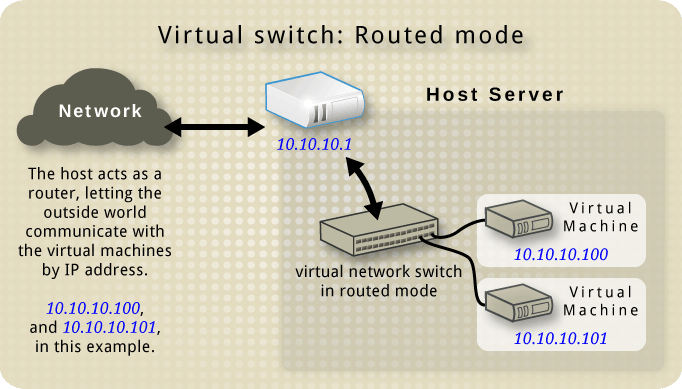
\includegraphics[width=4in]{figures/libvirt_routed_mode.png}
~\caption{Libvirt routed network. \cite{libvirt_networking}}
\label{figure3.1}
\end{figure}

With routed mode, the bridge is connected to the physical host LAN, passing guest network traffic back and forth without using NAT. This bridge sees the Ip in each packet and decides what to do. This mode gets all virtual machines in the subnet, routed through the bridge. The downside is that it is necessary to configure routers in order to get full access to the physical network. See Figure \ref{figure3.1}.

Also Epfiot takes benefit from Libvirt managed network because it has a DHCP feature that allows to generate virtual machine Ip addresses, making the effort of networking easy through dynamic network cards.

At this point, kernel parameters such as IP forwarding, and the proper NAT rules should be configured. Epfiot project comes with a set of networking script that makes this task easier.


\subsection{Tested Hardware}
\label{makereference3.1.3}
\subsubsection{Board}

In the execution of the project has been used the Intel NUC NUC5i5RYK with all the requirements below. It is a designed computer proposed by Intel which focuses on a high performance and small size.
Those characteristics fits perfectly with the Edge computing context, that is the reason to be selected as the board for this project.

Check the next table for more specifications of the device:

\begin{table}[H]
    \begin{center}
    \begin{tabular}[b]{|l|l|}
        \hline
        \textbf{NUC5i5RYB} & \\
        \hline
        Internal drive & M.2 SSD\\
        Processor & Intel® Core™ i5-5250U \\
        Cores	 & 2\\
        Threads & 4\\
        Base Frequency & 1.60 GHz\\
        Turbo Frequency & 2.70 GHz\\
        Memory size & 16 Gb\\
        Memory Type & DDR3L-1333/1600 1.35V SO-DIMM\\
        Memory Bandwitcth & 25.6 GB/s\\
        Memory Channels & 2\\
        Max DIMMS & 2\\
        Graphics &  Intel® HD Graphics 6000\\
        USB ports & 6\\
        Vtx & yes\\
        Vtd & yes\\
        \hline
    \end{tabular}
    \caption{Intel Nuc 5 specifications. ~\cite{nuc_specs}}
    \label{table1}
   \end{center}
\end{table}

\subsubsection{Usb accelerator}
As explained in this section \ref{makereference1.1}, Epfiot provides to the user the experience of using virtual machines connected to real usb accelerators, taking advance of the compute performance when realizing inference.

New Google coral was used in the project. Coral is a complete toolkit to build products with local AI. The on-board Edge TPU coprocessor is capable of performing 4 trillion operations per second (TOPS), using 0.5 watts for each TOPS.

Check the next table for more specifications of the device:

\begin{table}[H]
    \begin{center}
    \begin{tabular}[b]{|l|l|}
        \hline
        \textbf{Google Coral} & \\
        \hline
        ML accelerator & Google Edge TPU coprocessor\\
        Connector & USB 3.0 Type-C\\
        Dimensions & 65 mm x 30 mm\\
        \hline
    \end{tabular}
    \caption{Google coral specs ~\cite{coral_specs}}
    \label{table1}
   \end{center}
\end{table}


Notice that there are several Usb accelerators that could work with Epfiot solution similar to Google Coral, this device is used in this project with a test purpose.

\begin{figure}[h!]%t=top, b=bottom, h=here
\centering
    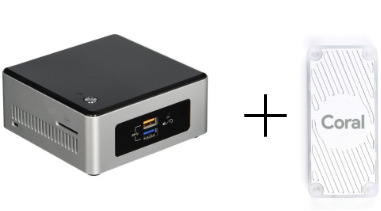
\includegraphics[width=4.5in]{figures/hardware.png}
~\caption{Devices used in Epfiot.}
\label{figure3.2}
\end{figure}
\newpage

\section{Appliance}
\label{makereference3.2}
The most important part of the Epfiot project relies in the Appliance. A virtual machine has been prepared with for the sake of serve a custom application that has been designed, developed and implemented thinking in this edge computing particular scenario.

This appliance running Epfiot, will be responsible of managing virtual machines, altogether with the devices connected to the host (usb accelerators), providing a multi-tenant environment, storing a persistent model, bringing a secure interface to the user among other things.

You can find some more details regarding these technologies of the development process in the next sections. The architecture of the application will be discussed in the next chapter.

\subsection{Operating System}
\label{makereference3.2.1}
\textbf{Alpine Linux} is the selected appliance for the operating System. It is a security-oriented, lightweight Linux distribution based on musl libc and busybox.
The decision was made taking into account the small footprint that the image leaves after installing Alpine and the resulting low consumption. 

For holding the image the \textbf{qcow2} format was selected, stands for 'Copy on Write' a very common term in the computer science field and uses a disk storage optimization strategy that delays allocation of storage until it is actually needed. Basically the image will grow only if the mounted file system needs more space. This is the format used not only for the application, but also for all virtual machines that Epfiot would manage.

\begin{figure}[h!]%t=top, b=bottom, h=here
\centering
    
\includegraphics[width=3in]{figures/alpine.png}
~\caption{Alpine Linux logo}
\label{figure3.3}
\end{figure}
\newpage


\subsection{Epfiot Package}
\label{makereference3.2.2}

Once the host part is covered and a virtual machine created with the operating system selected, it is time to explain the most complex part of the project, the Epfiot software, a custom package that has been made exclusively for this thesis. 

A brief scheme of the Epfiot appliance in the overall architecture of the project covered in this chapter is shown in the Figure \ref{figure3.3}.

\begin{figure}[h!]%t=top, b=bottom, h=here
\centering
    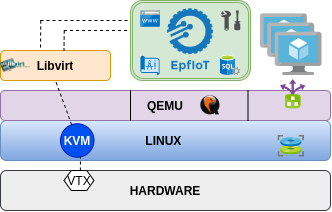
\includegraphics[width=5.5in]{figures/Epfiot_appliance.png}
~\caption{Epfiot appliance overview}
\label{figure3.3}
\end{figure}

The Epfiot package is a service that runs in the appliance that is composed by two major components:
\begin{itemize}
    \item Epfiot main application: \url{https://github.com/Semedi/epfiot}
    \item Epfiot Bootstrap Service: \url{https://github.com/Semedi/epfiot_bootstrap}
\end{itemize}

This subsection will explain the underlying technologies used in both components. On the other side, this will be used as an introduction for Chapter ~\ref{makereference4}. 
\newpage

\subsubsection{Epfiot Main application}

The Epfiot Main application is the heart of the project, its a piece of Software built from scratch that aims to fill all the purposes related in Chapter ~\ref{makereference1.3}. Before performing a deep dig into the architecture and the API interface of the project, main technologies will be arranged in order to grant a clear view to the reader.

\textbf{Dependencies}

\begin{enumerate}    
  \item alpine-sdk
  \item libvirt-dev
  \item libvirt-qemu
  \item cdrkit
  \item golang > 1.10.4
  \begin{enumerate}
    \item Epfiot
    \item libvirt-go
    \item net-http
    \item graphql-go
    \item gorm
    \item libvirt-go-xml
    \item ...
  \end{enumerate}

\end{enumerate}
The whole application has been developed using ~\textbf{git} as a version control system and hosted on Github. 
\textbf{Golang} was the selected language for this application. Go is an open source programming language that makes it easy to build simple, reliable, and efficient software.
Since Epfiot is a complex systems software and it is imperative that golang main purpose is to bring into the community an easy systems languaje, easy to learn, Golang was set as the best choice for developing Epfiot.

\begin{figure}[h!]%t=top, b=bottom, h=here
\centering
    
\includegraphics[width=3.0in]{figures/golang.png}
~\caption{Golang logo \cite{golang}}
\label{figure3.4}
\end{figure}

\newpage
Some of the advantages of using Golang that benefits Epfiot are:

\begin{itemize}
    \item Language Design: unlike other languages like C++, the designers of the language made a conscious decision to keep the language simple and easy to understand.
    \item Binaries: allowing the maintainer to administer a compiled version of the software. In this case the whole appliance is provided but it is possible to download the standalone epfiot distribution and install it in any x86 platform.
    \item Powerful standard library: As a system language this feature allow the developer to perform system calls and io operations in a safer way.
    \item Static Typing: Saving time debugging run-time errors.
    \item Concurrency Support: Ideal for a multi-tenant edge computing service.
    \item Package Management: Making easy to deal with dependencies.
\end{itemize}

Knowing the foundations stones of the project, it's time to show some key technologies:

\textbf{Libvirt, Qemu, KVM}: At this point these concepts should be very clear. The host operating system must have the Libvirt daemon running in the background (it is recommended to have the service enabled on systemd). In the appliance side, libvirt-qemu and libvirt-dev are needed. libvirt-qemu is a client of the libvirt daemon, by the other hand libvirt-dev contains the proper development headers. Libvirt-go which is a golang library is the binding for those headers, allowing the developer to build libvirt-tools using golang.

Libvirt uses xml for template definitions, which means that every resource created with libvirt must exist in a xml form. Managing templates with XML is a tedious thing, that's why libvirt-go-xml is brought into scope. This library handles the complex xml operations for building the document leaving behind a much simpler interface. Epfiot uses this library for building the templates. Those templates are sent to the host daemon using the libvirt client. Finally the libvirt daemon in the host side, knows how to instantiate the templates emulating the hardware on QEMU and granting kvm hypervisor capabilities for managing the guest.

\begin{figure}[h!]%t=top, b=bottom, h=here
\centering
    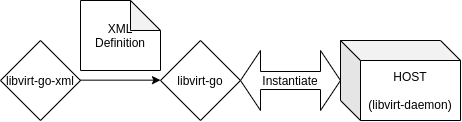
\includegraphics[width=3.9in]{figures/libvirt-xml.png}
~\caption{Libvirt basic scheme}
\label{figure3.4}
\end{figure}

\newpage

Libvirt ~\cite{libvirt_rpc} includes a basic protocol and code to implement an extensible, secure client/server RPC service. That is why Epfiot is able to communicate with the host in order to perform vm operations.
Trying to get a secure environment, Epfiot uses this rpc protocol tunneled over ~\textbf{SSH}. Epfiot takes profit of this situation using ssh for other mandatory tasks such as file system operations on the host machine.

Virtualization basics has been covered, let's move to net-http part.
\textbf{Net-http and graphql-go} correspond to Epfiot's service module. This module will be covered in detail all together with the others components in the next chapter, however, the technologies regarding this module will be explained below.

Golang languaje provides a good library for making http servers. Epfiot uses this library in order to build an interface to the end-user. At the time of building this interface, the most common design is usually famous REST API, nevertheless, a new technology was discovered replacing REST.
\textbf{GraphQL} ~\cite{graphqh_paper} is a framework with a query languaje that is used to express the data retrieval request issued to Web servers. This query languaje will behave taking into acount an schema that the developer should define.

Graphql gives clients the power to ask for exactly what they need and nothing more, makes it easier to evolve APIs over time, and enables powerful developer tools. These characteristic makes graphql very suitable for IoT, building this kind of service will save a lot of time since it does not require the design of new endpoints for every operation that the creator wants to expose.

Graphql-go is a graphql implementation in go, Epfiot uses this library to build a service module that serve as a http interface for user interaction. Epfiot has a schema for graphql that will define the end-user interaction with the system. More details about this schema can be found at Chapter ~\ref{makereference5}.

\begin{figure}[b!]%t=top, b=bottom, h=here
\centering
    
\includegraphics[width=4.5in]{figures/graphql.png}
~\caption{Graphql icon}
\label{figure3.5}
\end{figure}
\newpage

Finally in this section is worthed to appoint the persistence model.
\textbf{Gorm} is a golang library to work over this situation. It provides some fantastics features as a complete ORM model, Associations, Hooks, Transactions, SQL builder...

Epfiot uses Gorm in order to build a persistent model that a multi-tenant virtualization service should meet. This model is stored in a sql database. For development purposes \textbf{sqlite3} is the desired option, but for production environments is recommended to use Mariadb/Postgre.

\subsubsection{Epfiot Bootstrap service}

In order to bring some fancy IoT features into Epfiot, another piece of software was developed. The Epfiot Bootstrap service is a project that brings the \textbf{Lightweight M2M} protocol into this edge ecosystem.

\textbf{LWM2M} ~\cite{lwm2m_paper} is a Open Mobile Alliance standard that provides device management and service enablement capacities for managing IoT devices.
This protocol provides a light and compact secure communication interface along with an efficient data model. It is composed by LWM2M Client (M2M device) and a LWM2M Server (M2M platform), a client-server architecture in the top of CoAp using UDP/SMS as transport bindings. The architecture main's target is constrained devices that require an efficient bandwidth usage. ~\cite{IEE:lwm2m:2015}

Some features provided by LWM2M are the following:
\begin{itemize}
\item \textbf{Bootstrap}: LWM2M Bootstrap Server is able to manage keying, acess control and configuration of a device and enrol it with a LWM2M Server.
\item Device Discovery and Registration: The device (LWM2M client) permits the server (LWM2M server) know its existence.
\item Device management and service Enablement: allows LWM2M server to perform device management, sending operations to the client.
\item Information Reporting: Allows L2M2M to report information to the server.
\end{itemize}

The Epfiot Bootstrap service, which as its name suggest, is a Bootstrap server working with LWM2M that will handle the device bootstrapping phase, allowing those devices to register with normal LWM2M, being in this case the virtual machines.

The decision of creating a different project instead of performing a direct integration in the main package was made considering that L2M2M is a young protocol and find a valid implementation turnet into a very difficult task.
\newpage

Exploring possibilities for the project's implementation, it was decided to use \textbf{Wakaama}, an implementation made by Eclipse Foundation of the Open Mobile Alliance's LighWeight M2M protocol written in C, designed to be portable on POSIX compliant systems.

\begin{figure}[h]%t=top, b=bottom, h=here
\centering
    
\includegraphics[width=4.5in]{figures/Wakaama.png}
~\caption{Wakaama icon}
\label{figure3.6}
\end{figure}

The whole project can be found at: \url{https://github.com/eclipse/wakaama}, this project provides the Lwm2m for the C languaje and a few examples about LWM2M components such as bootstrap server, server, client... Epfiot has forked this implementation to build a custom bootstrap server that will work along the Epfiot main package to provide those capabilites to the project.

This package will listen to Epfiot requests in order to register devices and machines imported directly from the ORM model previously discussed.


\newpage
\section{Tuned image}
\label{makereference3.3}

The last section of this chapter introduces another image that is not the principal appliance. This tuned image is built specifically for the Epfiot project and is the base image that the virtual machines spawned by Epfiot will use. It's the only choice at the moment, any client using Epfiot is free to use whatever OS image they prefer, however, if you want to take advance of all Epfiot features, the main recommendation is to use the already prepared image, otherwise you would need to install certain components by yourself.

This part shows the content of this base image.
\begin{itemize}
    \item Ubuntu 18.04 as operating system.
    \item Cloud-init for instance initialization.
    \item LWM2M server enabled over websocket
    \item TPU runtime for google coral accelerator
    \item example projects
\end{itemize}

\begin{figure}[h]%t=top, b=bottom, h=here
\centering
    
\includegraphics[width=2.0in]{figures/cloud-init.png}
~\caption{cloud-init icon}
\label{figure3.6}
\end{figure}

Ubuntu is the elected operating system due to it is the Linux distribution that support a wide variety of environments, for example the TPU runtime package needed for the Google Coral accelerator works perfectly with Ubuntu and 18.04 is a stable version.

\textbf{Cloud-init} is a service installed inside the image that allows Epfiot to provide vm configuration bootstrapping. When a virtual machine is created, Epfiot asks to the user for a configuration, like for example username and password. Epfiot creates a CDROM owned by the virtual machine, the cloud-init service will read this CD-ROM at boot-time executing the configuration defined by the user. Cloud-init was created by Canonical and it's adopted in many companies and institutions such as AWS with the same purpose of Epfiot.

LWM2M server was already explained in ~\ref{makereference3.2.2}, remembering the Wakaama project, a LWM2M server has been compiled. This binary is enabled as a service at vm boot time and provided to the user with a websocket! Some adjustments are still required but this grant the possibility of having a platform that is able to register your devices in an automatic way.

With the components previously discussed, the Google Coral TPU runtime is installed with the image, allowing to perform inference operation using real hardware. Remember that the machine is already prepared to have a device and KVM is the responsible of perform the passthrough operation so, you will experience the use of a normal machine with a connected device handled by udev.

How this service is able to communicate with the main Epfiot package will be explained all together with the application's architecture in the next Chapter. 







